\documentclass[aps,prl,reprint]{revtex4-1}
\usepackage{blindtext}
\usepackage{ mathrsfs,placeins }
\usepackage{cleveref}
\usepackage{amsmath,wrapfig}
%\usepackage[justification=centering]{caption}
\usepackage{graphics,setspace,enumitem,graphicx,textpos}
\begin{document}
\bibliographystyle{plain}
\title{	Analysis of Matter and Dark Energy Content of the Universe via MCMC fitting of Type Ia Supernova Data}
\author{Delilah Gates}
\email{dgates@g.harvard.edu}
\author{Ann Wang}
\email{annwang@g.harvard.edu}
\affiliation{Harvard University}
%\begin{spacing}{1.2}
\begin{abstract}
%Something about cosmology abstract TBA
\end{abstract}
\maketitle
\section{I. Introduction}
One compelling question in cosmology research today is why the energy budget of the universe is dominated by dark energy, acting as a ``negative pressure" driving the universe further and further apart. Since the observation of Type Ia supernovae showed that the universe was expanding at an accelerated rate, dark energy research has been an active area of study \cite{riess_sn}. One ``form" of dark energy that could cause the universe to expand at an accelerated rate is a cosmological constant.

The cosmological constant was first introduced by Einstein in his equations of general relativity to allow for a static universe by choosing the constant so that its effect canceled the effect of gravitation. However, Einstein later removed the cosmological constant because such a universe is unstable. In 1929, Hubble discovered the linear relationship between distances of galaxies and their redshifts \cite{Straumann:2002he}. Lemaître then showed that Hubble's results fit with the Friedmann-Lemaître-Robertson-Walker (FLRW) model of an expanding universe which was based off of Einstein's GR equations. However, when Hubble's results were interpreted in the context of the universe expanding at a constant rate, his findings suggested that the universe was much too young (less than half the age of Earth as measure via radioactive dating). To reconcile Hubble's results with the age of the universe, Eddington and others suggested the reintroduction of the cosmological constant, but with a value large enough to detect an accelerated expansion of the universe today \cite{Straumann:2002he}. 

While Hubble measured redshifts and distances of galaxies, today such measurements are also done with Type Ia Supernovae. Type Ia Supernovae are good candidates for the measurement of the expansion of the universe because they are believed to be standard candles \cite{shocker}. Thus, the difference in the distance moduli of two supernovae can be attributed to their distances (and experimental error and noise) as opposed to differences in the radiation given off by the two objects. While supernovae data is not the only data supporting dark energy and the expansion of the universe, it has been generally accepted that supernovae data supports the claim \cite{riess_sn,sdss}. However recently, a study by J.T. Nielson et al. \cite{shocker} claimed, analyzing a larger set of supernovae data, that there was little evidence for an accelerated rate of expansion. We reanalyze the same data set and present our findings here.
\section{II. Background}
To compare results, we use data from the Joint Lightcurve Analysis (JLA) catalog \cite{sdss}, which uses the Spectral Adaptive Lightcurve Template 2 (SALT2) approach to characterize Type Ia Supernovae \cite{salt2}. This combines the recent SDSS-II survey along with several past surveys from other experiments \cite{sdss}. There are several versions of the covariance matrix for the distance modulus; we use the covmat\_v6 version along with the corresponding code to convert the covariance data from FITS format \cite{fits} to a matrix format given $\alpha$, $\beta$ (see later $\mu$ equation), which was provided at http://supernovae.in2p3.fr/sdss\_snls\_jla/ReadMe.html. 
\par The data provides us with several characteristic values for every SN Ia: the heliocentric redshift $z_{hel}$, the CMB frame redshift $z_{CMB}$, the apparent magnitude $m_B$, the shape parameter from SALT2, $x_1$, the color correction $c$, and the host stellar mass $M_{stellar}$ \cite{sdss}. Using these parameters, we can define a distant modulus which can be compared to a value expected by a certain cosmological model. This distance modulus is given by \cite{sdss}: 
\begin{equation}
\mu = m_B - M + \alpha x_1 - \beta c
\end{equation}
The M, or absolute magnitude, is dependent on the host galaxy, so we follow the prescription in \cite{sdss}, where if $M_{stellar} < 10^{10} M_{\odot}$, then $M_B = M_B'$, otherwise, $M_B = M_B' + \Delta_M$. 

SALT2, a Spectral Adaptive Lightcurve Template 2, was trained by J. Guy et al on the light curves of large sets of supernovae to produce the above model of the distance modulus \cite{salt2}. The SALT2 model is used by J.T. Nielson et al. (who claim marginal evidence for universal accelerated expansion via supernova data) and M. Betoule et al. (who claim supernovae data suports universal accelerated expansion) \cite{shocker,sdss}. SALT2 is now widely used after it was shown that for a flat $\Lambda$CDM universe, it gives a 10\% improvement on the error in $\Omega_M$ as compared to the first SALT model trained on supernovae data \cite{salt2}.

For comparison, using the density parameters ($\Omega_m$, $\Omega_{r}$, $\Omega_{\Lambda}$) and curvature ($\Omega_k$) of a cosmological model one can calculate the theoretical distance modulus of an object at a certain redshift as follows:  
$$E(z)=\sqrt{\Omega_{r}(1+z)^4 + \Omega_m(1+z)^3 + \Omega_k(1+z)^2 + \Omega_{\Lambda}} $$
$$d_L(z)=\frac{c}{H_0} {\int_0}^z \frac{dz'}{E(z')} $$
\begin{equation}
\mu = 25 + 5\;\text{log}_{10} \left( \frac{d_L(z)}{\text{Mpc}} \right) 
\end{equation}

For our flat universe, given the heliocentric and CMB redshifts, we can rewrite the luminosity distance as \cite{miao}:
$$d_L(z_{hel},z_{cmb})=\frac{(1+z_{hel}) c}{H_0}{\int_0}^{z_\text{cmb}} \frac{dz'}{E(z')}$$

\section{III. Methods}
We perform a likelihood analysis using MCMC methods. Our code can be found online at https://github.com/deagates/CosmologySNProject.
\subsection{Case for MCMC method}
MCMCs use Bayesian statistics to access the likelihood of various values for parameters in a model given observed data to find the most likely values of a model.
To initialize our MCMC, random values are drawn from a distribution known as the prior for the parameter values of a model and recorded. Then the probability of the model given the data set is calculated via some pre-specified likelihood function. For the next step, new temporary parameter values (close to the previous ones and randomly drawn from some specified jumping distribution) are chosen and the probability of these values is calculated. If the probability with the temporary values is bigger than the probability with the original values, the new values are rejected and the old values are once again recorded. If the probability with the temporary values is smaller than the probability with the original values the new values are accepted with a probability equal to the ratio of the new likelihood to the old. If the new values are accepted they replace the previous values. The process is then repeated with the new parameter values \cite{lecture}.

Once the MCMC has been run long enough to converge, this gives a string of parameter values that are concentrated around the values that are most likely. One can then make inferences from this string of parameters. 

\subsection{MCMC details}

\par We adopt the likelihood function described in \cite{sdss}, which is defined to be $$\mathscr{L} = \text{exp}(-\frac{\chi^2}{2}) $$ where$$\chi^2 = (\hat{\mu}-\mu_\text{model})^\dagger C^{-1} (\hat{\mu}-\mu_\text{model}),$$  with C as the covariance matrix, and $\hat{\mu}$ and $\mu_\text{model}$ are calculated using (1) and (2) respectively . For simplicity and comparability with J.T. Nielson et al., we take $\Omega_r$ the radiation density parameter of the universe to be 0, further justified by the fact that the measured radiation density parameter of today is very small, and we assume the universe is flat ($\Omega_k = 0$). This leaves us with the constraint that $\Omega_m + \Omega_{\Lambda} = 1 $. We have five model parameters ($\Omega_m$, $\alpha$, $\beta$, $M'_B$, and $\Delta_M$) that our MCMC varies to try to maximize the likelihood.
\par The covariance matrix, provided at the aforementioned database, is composed of several errors. Equation (11) of \cite{sdss} describes the covariance matrix as: \begin{math}  \newline \newline  \indent \indent \indent \indent  C_\eta = C_{\text{stat}} + (C_{\text{cal}} + C_{\text{model}} + C_{\text{bias}} \newline
\indent \indent  + C_{\text{host}} + C_{\text{dust}})_{\text{reevaluated}} + (C_{\text{pecvel}}+C_{\text{nonIa}})_{\text{C11}}.\end{math}
\newline \par Included in this matrix are: the statistical uncertainties encompass the light-curve fit uncertainties, the photometric calibration uncertainties, uncertainties associated with the light-curve model, uncertainties associated with selection biases from the surveys, the uncertainties of the host masses, an uncertainty to limit sensitivity to Milky Way dust extinction, and two uncertainties taken from the compilation of all of the supernova data not from SDSS (i.e. SNLS, HST, etc.) from Conley et al. \cite{c11}. This is then combined to calculate the covariance matrix of the distance modulus, which is defined in eq. 13 of \cite{sdss} as follows:
$$C = A C_\eta A^\dagger + \text{diag}(\frac{5\sigma_z}{z \text{log} 10})^2 + \text{diag}(\sigma_\text{lens}^2) + \text{diag}(\sigma_{\text{coh}}^2). $$
This combines more uncertainties on the redshift, additional effects from gravitational lensing, and a catch-all term for other uncertainties on the magnitudes. \cite{sdss} claims that the catch-all estimation, which in effect replaces a $\sigma_\text{int}$ which Conley et al. use, is less biased towards a specific cosmological model. We use the final $C$ matrix in the calculation of our likelihoods. 

\par We ran our MCMC analyzer for several iterations, each in excess of 10,000 steps. The prior distributions on the five fit parameters were all flat, with bounds as given in table \ref{bounds}. These regions are \textit{roughly} centered around the reported best-fit parameter values of \citep{sdss}.
\par After the initial random draw of the parameter, the next iterative parameter values were picked using a random draw from normal distributions centered around the current parameter values (with a $\sigma$ of 0.5 for $\Omega_M$ and a $\sigma$ of 0.8 for the nuisance parameters) that were truncated at the aformentioned parameter bounds. These sigma values were hand-tuned by running several test runs and looking at the trace plots to ensure good ``mixing" \cite{MC}. Trace plots from one of the runs are shown in \cref{fig:trace}. 
\onecolumngrid


\begin{figure}[t!]
 \centering
 \includegraphics[width=.8\textwidth]{../plots/SN_trace.pdf}
 \centering
\caption{\label{fig:trace}An example of a $\alpha$, $\beta$, $M'$, $\Delta_M$, and $\Omega_m$ trace plots for one of the MCMC iterations.}
\end{figure}
\twocolumngrid
Ultimately, we ran our MCMC for several iterations (with the aforementioned bounds and $\sigma$ values). To be sure of convergence we removed the first 10,000 values of each iteration. Then we aggregated the left over values from each iteration into one large data set. This generates a set of 41,528 points. (Not all the iterations were the same length with the last two having been short in the interest of time.) It is this large aggregated data set which we analyze next.

\begin{table}
\begin{center}
\begin{tabular}{ |c|c|c| } 
 \hline
 \textbf{Parameter} & \textbf{Upper Bound} & \textbf{Lower Bound} \\ 
 $\Omega_M$ & 0 & 1 \\ 
 $\alpha$ & -1 & 4 \\ 
 $\beta$ & 1 & 6 \\ 
 $M'_B$ & -21 & -17 \\ 
$\Delta_M$ & -2 & 1 \\ 
 \hline
\end{tabular}
\caption{Constraints on parameter values during fitting.}\label{bounds}
\end{center}
\end{table}
\FloatBarrier
\onecolumngrid

\begin{figure}
\includegraphics[width=0.8\textwidth]{../plots/SN_hist.pdf}
\caption{\label{fig:hist}The aggregated distribution of values of $\alpha$, $\beta$, $M'$, $\Delta_M$, and $\Omega_m$ from the MCMC, throwing out the first 10,000 steps in each run.}
\end{figure}
\twocolumngrid
\begin{table}[t]
\begin{center}
\def\arraystretch{1.5}
\begin{tabular}{ |c|c|c|c|c| } 
 \hline
 \textbf{Parameter} & \textbf{Avg.} & \textbf{Wgtd. Avg.} & \textbf{Med.} \\ 
 $\Omega_M$ & 0.485 & 0.468 & $0.481^{+0.321}_{-0.312}$\\ 
 $\alpha$ & 0.319 & 0.287 & $0.293^{+0.384}_{-0.342}$\\ 
 $\beta$ & 4.309 & 4.172 &  $4.516^{+0.989}_{-1.473}$\\ 
 $M'_B$ & -19.368 & -19.361 & $-19.382^{+0.626}_{-0.603}$ \\ 
$\Delta_M$ & -0.303 &-0.289 & $-0.268^{+0.701}_{-0.780}$ \\
 \hline
\end{tabular}
 \caption{Final MCMC values.}\label{tblv}
\end{center}
\end{table}

\begin{figure}
 %\centering
 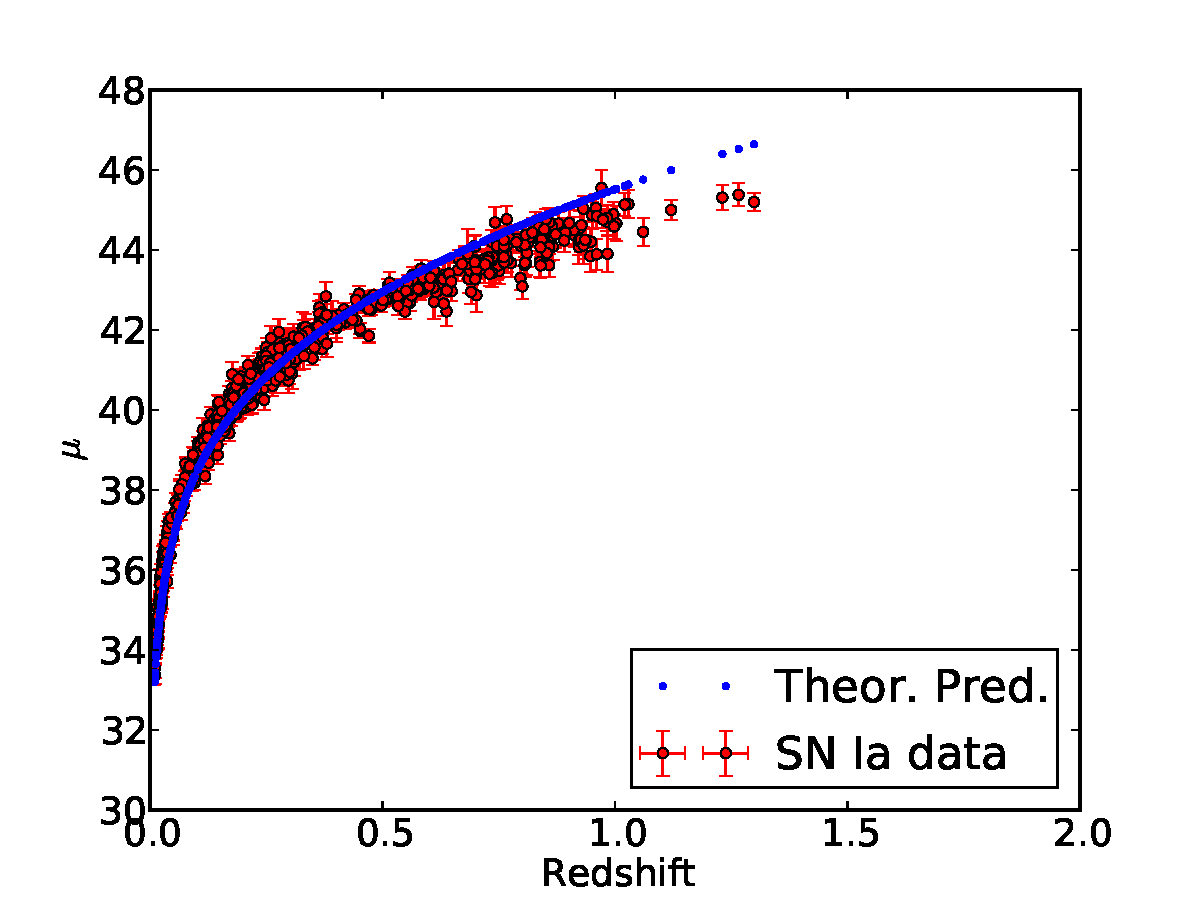
\includegraphics[width=0.5\textwidth]{../plots/mu.pdf}
\caption{\label{fig:mu}The distribution of distance modulii versus redshift for the SN Ia points used in the analysis from the JLA catalog. The $\mu_\text{model}$ distribution predicted by our best-fit value (using weighted averages) of $\Omega_l$, $\Omega_m$ is overlaid in blue.}
\end{figure}

\section{IV. Analysis} 
Our final values are quoted in the final table (see Table \ref{tblv}). Errors were approximated as 68\% around the median value of the distribution. The distributions of the points that went into these calculations are the histograms of the aggregated dataset given in \cref{fig:hist}.
Despite following a method similar to that of \cite{sdss}, we find different values for $\Omega_m$, which they report to be 0.295 $\pm$ 0.034. Visually, we can inspect the expected data points given by our parameter fit values in \cref{fig:mu}; we see some deviation from the data, especially near higher redshifts. Regardless of the discrepancy in the reported values, it is clear that the best-fit values we report are not consistent with a constant rate of expansion.
\section{V. Discussion}
Our approach follows the steps of \cite{sdss}, using the same likelihood function and fit parameters but does not recover extremely similar results. Areas of concern that may have negatively affected the results are the bounds on the parameters mentioned in table 1, the jumping functions in the MCMC, and the method of determining the final quoted values.

The ranges on the nuisance parameter draw regions were defined such that they encompassed the reported values of \cite{sdss}, as we expected the results to converge to similar numbers. However, from the trace plots and histograms it is apparent that, while the distributions for $\alpha$ and $\Delta_m$ look well-behaved (approximately normal distributions), it seems that the bounds on $\beta$ and $\Delta_m$ should have been expanded. One way we could have allowed for this is by not choosing truncated gaussians as the distributions for drawing new parameter values. Furthermore, the histogram distributions for $\beta$ and $\Delta_m$ could perhaps be improved by fine-tuning the sigmas of the nuisance parameter jumping distributions. We chose $\sigma = 0.8$ as not all the parameters should expect the same jumping distribution. For $\Omega_m$, a jumping distribution that is strictly between 0 and 1 is required since $\Omega_m$ cannot take values outside this range.

Not wanting to make to many assumptions about the shapes of our histograms, we reported the median, the average, and the weighted average values. Another way to conclude the most favorable values of $\alpha$, $\beta$, $M_B'$, $\Delta_m$, and $\Omega_m$, would be to fit the histograms to some distribution (e.g. a normal distribution, or a sum of two normal distributions) and report the values as the peaks and confidence levels given by the fit. This would, for example, have given us a higher value for $\beta$ because our asymmetric distribution has biased the final value. In future studies, to make a direct comparison with J.T. Nielson et al., our approach can be expanded to adopt their likelihood function. 
They employ an alternative likelihood function, which they define as \begin{align*}\mathscr{L} = |2\pi(C+A^T \Sigma_l A)|^{-1/2}\; \\
\times \text{Exp}[-(\hat{Z}-Y_0A)(C+A^T\Sigma_lA)^{-1}(\hat{Z}-Y_0A)^T/2],\end{align*} where $\Sigma_l = \text{diag}[\sigma_{M_0}^2,\sigma_{X_{1,0}}^2,\sigma_{C_0}^2,...],$ $A = ,$ $\hat{Z} = [\hat{m}_{B1}-\mu_1, \hat{x}_{11},\hat{c}_1,..]$, and $Y_0 = [M_0,x_{1,0},c_0,....]$. 
\par To make a more accurate comparison, this likelihood function should be implemented and compared directly to the $\chi^2$ likelihood function. Then, the authors' reported effect of the alternative likelihood measure could be evaluated while keeping all of the other conditions (such as the host stellar mass handling) the same. 

\subsection{An unexplained peculiarity}
In trying to diagnose problems with our MCMC, we came across a peculiar phenomenon we thought worth briefly mentioning. Plotting the $\chi^2$ values verse $\Omega_M$ of the aggregated data in \cref{fig:chi2}, $\chi^2$ never dips below $\approx$2 for all values of $\Omega_M$. Furthermore, there is an unexplained slope on the floor of the likelihood across varying values of $\Omega_m$. It is not apparent if this problem can be alleviated by the aforementioned changes. 

\begin{figure}
% %\centering
 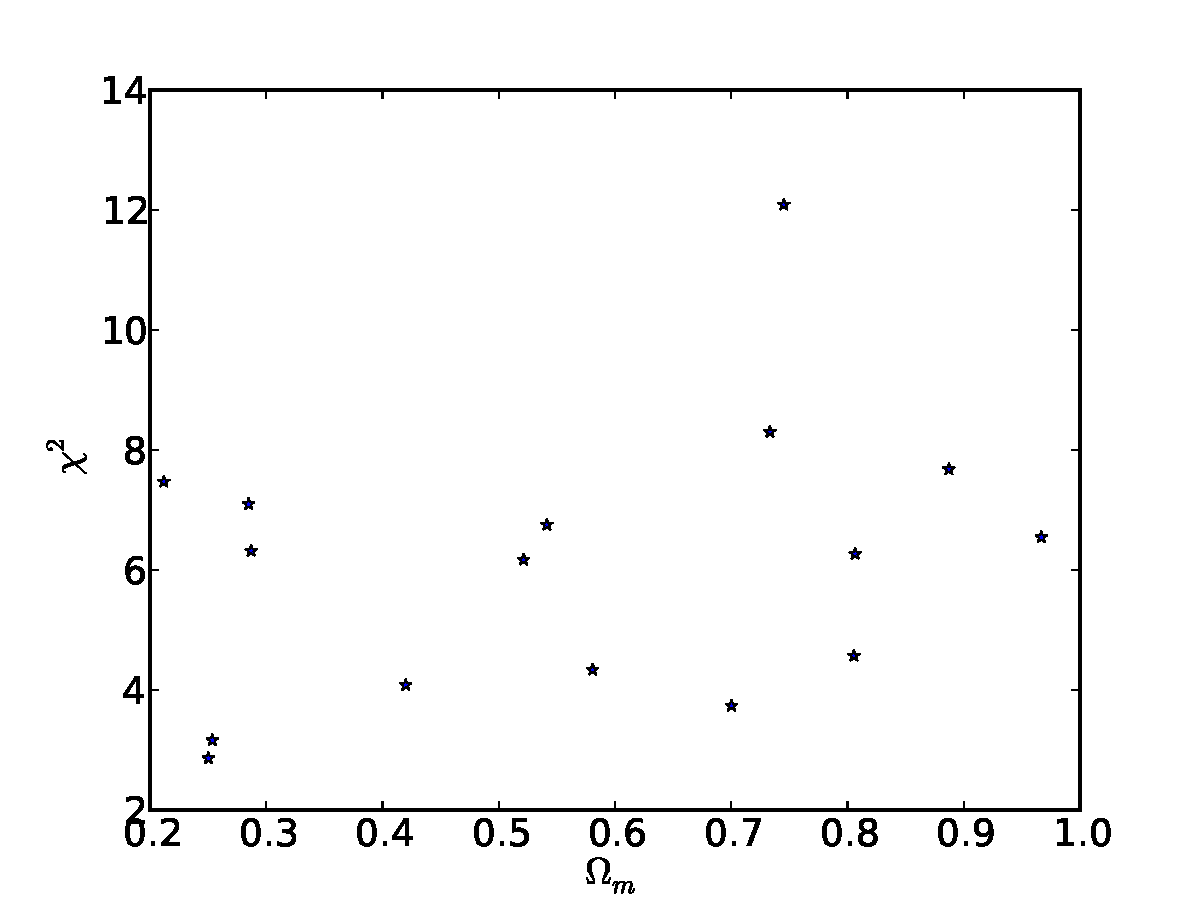
\includegraphics[width=0.5\textwidth]{../plots/om_chi.pdf}
\caption{\label{fig:chi2}The values of $\Omega_M$ from each MCMC versus the corresponding $\chi^2$ values.}
\end{figure}
 
\bibliographystyle{apsrev4-1} % Tell bibtex which bibliography style to use
\bibliography{cosmo_bib} 
\end{document}
